\documentclass{report}
\usepackage{minted}
\usepackage{verbatim}
\usepackage{fullpage}
\usepackage{etoolbox}
\usepackage{lipsum}
\usepackage{graphicx}

\graphicspath{ {res/} }
\newcommand{\HRule}{\rule{\linewidth}{0.5mm}} 

\begin{document}
    \begin{titlepage}

        \center

        \textsc{\LARGE Universita' degli Studi di Messina}\\[1.5cm] 
        \textsc{\Large Networking course project}\\[0.5cm] 

        \HRule \\[0.4cm]
        { \huge \bfseries AutoSyncGen}\\[0.1cm]

        {\large \today}
        \HRule \\[1.5cm]
         
        \begin{minipage}{0.4\textwidth}
        \begin{flushleft} \large
        \emph{Author:}\\
        Vittorio \textsc{Romeo} % Your name
        \end{flushleft}
        \end{minipage}
        ~
        \begin{minipage}{0.4\textwidth}
        \begin{flushright} \large
        \emph{Professors:} \\
        Antonio \textsc{Puliafito}

        Giovanni \textsc{Merlino}
        \end{flushright}
        \end{minipage}\\[4cm]

        \vfill

        \begin{minipage}{\linewidth}
            \centering
            \begin{minipage}{0.35\linewidth}
                \begin{figure}[H]
                    \center
                    
\includegraphics[width=3cm, height=3cm]{logounime}
                    
                    http://unime.it
                \end{figure}
            \end{minipage}
            \hspace{0.27\linewidth}
            \begin{minipage}{0.35\linewidth}
                \begin{figure}[H]
                    \center
                    
\includegraphics[width=3cm, height=3cm]{logovee}
                    
                    http://vittorioromeo.info
                \end{figure}
            \end{minipage}
        \end{minipage}\\[3cm]
    \end{titlepage}


    \pagenumbering{gobble}
    \tableofcontents
    \newpage
    \pagenumbering{arabic}
    
    \chapter{Introduction}
        What is \emph{AutoSyncGen} and what is it trying to achieve?
    
        \section{Problem}
            Many networked applications require \emph{constant synchronization} between the server and the connected clients. 
            Software such as \emph{multiplayer online games} completely rely on the fact that a synchronized state is maintained between the server and the players.
            Other applications that are not reliant on state synchronization may still benefit from such a system. 
            A \emph{basic chatroom program}, for example, may use state synchronization to keep track of sent messages and allow newly-connected users to browse the message history.

            Implementing state synchronization is not a trivial task. It it usually required to define a simple protocol that \emph{explicitly handles} state synchronization for all data structures. 

            This is usually achieved by explicitly coding serialization behavior and explicitly defining how packets should be created and read for every synchronizable objects. Even for small applications, maintaining and expanding the code using a similar approach can become difficult quickly.

        \section{Solution}
            The solution proposed in this papers is \emph{AutoSyncGen}, a \emph{C++14} library written using \emph{modern and idiomatic code}.
            The library allows developers to quickly define synchronizable data structures, and automatically deals with \emph{object lifetime management}, \emph{serialization} and \emph{deserialization}, packet \emph{creation} and \emph{reading}.

            By quickly specifying how object memory should be managed and the types of the synchronizable fields, \emph{AutoSyncGen} generates code at \emph{compile-time} to keep track of the entire application state and generate synchronization requests and responses that send the smallest amount of data required to fully synchronize the clients to the server.

            \newpage

            Here's an example of a synchronizable data structure defined using the AutoSyncGen library.

            \begin{minted}[mathescape, linenos, numbersep=5pt, gobble=2, frame=lines, framesep=2mm]{cpp}
    // Synchronizable data structure representing a chat message.
    struct Message : syn::SyncObj
    <
        // The fields types are passed as a variadic type list.

        int,            // messageID
        std::string,    // author
        std::string     // contents
    >
    {
        // Field proxies are generated via macros for convenience.

        SYN_PROXY(0, messageID);
        SYN_PROXY(1, author);
        SYN_PROXY(2, contents);
    };
            \end{minted}

            A shorter (but more preprocessor-heavy) construct can be used, which reduces code repetition.

            \begin{minted}[mathescape, linenos, numbersep=5pt, gobble=2, frame=lines, framesep=2mm]{cpp}
    // Synchronizable data structure representing a chat message.
    SYN_DEFINE_SYNCOBJ
    (
        // Name of data structure.
        Message,

        // Tuple of synchronizable fields.
        (
            (int, messageID),
            (std::string, author),
            (std::string, contents)
        )
    );
            \end{minted}

            The library is structured in such a way that most of the user code can be \emph{shared between the client and the server}. 
            It is not necessary to re-define data structures or lifetime management instructions twice.

        \section{Technologies used}
            C++14, which is the latest official C++ standard, released in 2 March 2014 \emph{(paper N3936)}, is the language of choice for AutoSyncGen.
            Like C++11, this newer standard is a huge step forward for the language. \emph{Smarter memory managament}, \emph{automatic type deduction}, and countless new programming and metaprogramming features allow developers to write much safer and powerful code.
            C++11 and C++14 features make AutoSyncGen possible.

            On top of C++14 and its standard library, the \emph{SSV framework} is being used as well. This framework was completely written from scratch by me, \emph{Vittorio Romeo}, and is available under the open-source AFL3.0 license on GitHub.

            The \emph{SSVUtils} library, used throughout the whole program, features many heterogeneous self-contained modules: an efficient and modern handwritten JSON parser, a preprocessor metaprogramming module, a template metaprogramming module, automatic console formatted output for containers and user-defined types, efficient data structures (bimap, handle vector, growable arrays), advanced memory management facilities, type-safe variadic unions, handwritten templating system, filesystem management, easy benchmarking of portions of code, and much more.

            Two additional dependencies for AutoSyncGen are the \emph{SFML} library, which offers lightweight abstraction over sockets and packets, and the \emph{SSVStart} library, part of the SSV framework, which extends the functionality of SFML and wraps some of its C++03 abstractions with more modern and safer C++14 constructs.
    
    \newpage

    \chapter{Network module}
        AutoSyncGen is divided in two main modules. 
        The \emph{network module} deals with client/server abstraction and communication, and will be covered in this chapter.
        The \emph{synchronization module} deals with compile-time synchronization data structures generation and synchronization algorithms, and will be covered in the next chapter.

        \section{SFML}
            As mentioned in the previous chapter, SFML is one of the dependencies of AutoSyncGen. 
            SFML offers convenient and type-safe wrappers over basic networking constructs such as \emph{sockets} and \emph{packets}.

            AutoSyncGen's network module extensively uses these abstractions to allow cross-platform compatibility and additional safety.

            \begin{minted}[mathescape, linenos, numbersep=5pt, gobble=2, frame=lines, framesep=2mm]{cpp}
    // SFML offers an `IpAddress` data structure that that can be initialized from strings.
    using sf::IpAddress;
    
    // SFML offers a `Packet` object that can be filled/emptied using stream operators.
    using sf::Packet;

    // SFML offers an `UdpSocket` class that properly manages and abstracts the memory 
    // and functionality of an UDP socket.
    using sf::UdpSocket;
            \end{minted}

            Just to clarify how convenient these abstractions are, here's a small code example that shows \emph{sf::Packet} usage.

            \begin{minted}[mathescape, linenos, numbersep=5pt, gobble=2, frame=lines, framesep=2mm]{cpp}
    int x{5};
    std::string y{"hello!"};
    double z{2.52};

    sf::Packet toSend;
    toSend >> x >> y >> z;

    // Send packet through the UDP socket...

    int outX; 
    std::string outY;
    double outZ;
    
    sf::Packet received;
    received << outX << outY << outZ;
            \end{minted}

            SFML is open-source, cross-platform and free.

        \section{Packets}
            AutoSyncGen uses a simple but effective protocol for data synchronization, which requires some special packets.

            \subsection{Packet types}
                Packet types are defined using \emph{C++11 enum classes}, which are type-safe enumeration types that cannot be implicitly converted to their underlying representation.

                \subsubsection{CtoS enumeration}
                    This enumeration holds the packet types that are sent from the client to the server.

                    \begin{minted}[mathescape, linenos, numbersep=5pt, gobble=2, frame=lines, framesep=2mm]{cpp}
    enum class CtoS : NType
    {
        // Request to establish a connection to the server
        ConnectionRequest = 0,      
        
        // Ping to avoid timing out with the server
        Ping = 1,                   

        // Request to sync data with server
        SyncRequest = 2,            
        
        // Informs the server that the syncronization was successful
        SyncSatisfied = 3,         

        // Custom data packet
        Data = 4,                   
    };
                    \end{minted}

                \subsubsection{StoC enumeration}
                    This enumeration holds the packet types that are sent from the server to the client.

                    \begin{minted}[mathescape, linenos, numbersep=5pt, gobble=2, frame=lines, framesep=2mm]{cpp}
    enum class StoC : NType
    {
        // Accept a requested client connection, assigning the client a CID
        ConnectionAccept = 0,       
        
        // Decline a client's requested connection
        ConnectionDecline = 1,      

        // Satisfy sync request (if the client's revision is behind)
        SyncRequestSatisfy = 2,     

        // Sync not needed (client has the same revision as the server)
        SyncRequestUnneeded = 3,    

        // Sync request declined (overload/technical issue)
        SyncRequestDecline = 4,     

        // Custom data packet
        Data = 5,                   
    };
                    \end{minted}
            
            \subsection{Packet handling}
                Packets are automatically handled by the client and the server, using a switch.

                \begin{minted}[mathescape, linenos, numbersep=5pt, gobble=2, frame=lines, framesep=2mm]{cpp}
    void handle(RPT mType)
    {
        switch(mType)
        {
            case RPT::ConnectionAccept:
                handleConnectionAccept();
                return;
            case RPT::ConnectionDecline:
                handleConnectionDecline();
                return;
            // ...
        }
    }
                \end{minted}

                This implementation is fine for the current packet types AutoSyncGen uses, but can be changed to a lookup table or an array of function pointers if more packet types need to be added in the future.

        \section{SessionHost}

            Clients and servers are abstracted as \emph{SessionHost} classes in the network module.
            The \emph{SessionHost} classes defines data structures and functionality shared both by clients and servers.

            Every host has a dedicated extra thread for data and socket management.

\begin{minted}[mathescape, linenos, numbersep=5pt, gobble=2, frame=lines, framesep=2mm]{cpp}
    // `SessionHost` is a CRTP template class, to allow compile-time generation 
    // of appropriate data structures.
    template
    <
        // `struct` containing global synchronization settings.
        typename TSettings, 
        
        // Type of sent packets.
        typename TSPT, 
        
        // Type of received packets.
        typename TRPT, 

        // CRTP (curiously recurring template pattern) derived type.
        template<typename> class TDerivedBase
    > 
    class SessionHost
    {
        // Typedefs of data structures that depend on the template parameters.
        public:
            // CRTP type.
            using Derived = TDerivedBase<Settings>;

            // Packet types.
            using SPT = TSPT;
            using RPT = TRPT;
        
            // Synchronization classes.
            using Settings = TSettings;
            using SyncManager = typename Settings::SyncManager;
            using Diff = typename SyncManager::DiffType;
            using Snapshot = typename SyncManager::SnapshotType;

        private:
            // Name of the host.
            std::string name;
            
            // IP address of the host.
            IpAddress ip;

            // Port the host is listening on.
            Port port;

            // UDP socket of the host.
            UdpSocket socket;

            // Status of the host.
            bool busy{false};

            // Tries binding the socket to the specified port.
            void tryBindSocket();    

            // Tries forwarding the received packets to the underlying 
            // client/server implementation.
            void tryForwardReceivedPacket();
            
            // Function running in the receive thread, which keeps track
            // of the data receiving buffer and of the socket state.
            void receiveThread();

        protected:
            // Buffers that store received data and data that will be sent.
            Packet sendBuffer, recvBuffer;

            // `void` future offering a RAII wrapper for the host's thread.
            std::future<void> hostFuture;

            // IP of the sender of the last received data.
            IpAddress senderIp;
            
            // Port of the sender of the last received data.
            Port senderPort;
            
            // Synchronization manager.
            SyncManager syncManager;

            // Sends the content of the send buffer to the specified host.
            void sendTo(const IpAddress& mIp, const Port& mPort);

            // Builds a packet from a variadic argument list.
            template<SPT TType, typename... TArgs> void mkPacket(TArgs&&... mArgs);

            // Sets the state of the host.
            void setBusy(bool mBusy) noexcept { busy = mBusy; }

            // Pops data of type `T` from the receive buffer.
            template<typename T> auto popRecv();

        public:
            // Constructs the host using a specified name and port.
            // This function tries to bind the socket and start the dedicated thread.
            SessionHost(std::string mName, syn::Port mPort);

            // Getters.
            const auto& getName() const noexcept;
            const auto& getIp() const noexcept;
            const auto& getPort() const noexcept;
            const auto& isBusy() const noexcept;
            auto& getSyncManager() noexcept;
    };

    // Template typedef for the base `SessionHost` used by servers.
    template<typename TSettings> 
    using SessionServerBase = SessionHost<TSettings, PT::StoC, PT::CtoS, SessionServer>;

    // Template typedef for the base `SessionHost` used by clients.
    template<typename TSettings> 
    using SessionClientBase = SessionHost<TSettings, PT::CtoS, PT::StoC, SessionClient>;
\end{minted}

            \subsection{SessionServer}

                The \emph{SessionServer} CTRP derivation of \emph{SessionHost} requires additional data structures and algorithms to deal with client connections and storage of the client's latest synchronization state snapshots.

                \subsubsection{ClientHandler}

                    A \emph{ClientHandler} instance is created and managed for every client connected to the server.

\begin{minted}[mathescape, linenos, numbersep=5pt, gobble=2, frame=lines, framesep=2mm]{cpp}
    class ClientHandler
    {
        private:
            // Connect client ID. 
            // Assigned by the server.
            CID cid{nullCID};

            // IP and Port of the client.
            IpAddress ip;
            Port port;

            // Seconds until the client is timed out.
            int secondsUntilTimeout;
            
            // State of the client handler.
            bool busy{false};

        public:
            // Assumes the handler is not busy and binds it to a client with a
            // specific client ID, IP and Port.
            void bindToClient(CID mCID, const IpAddress& mIp, const Port& mPort);

            // Unbinds the handler from the client connection.
            void unbindFromClient();

            // Getters
            const auto& getCID() const noexcept;
            const auto& getIp() const noexcept;
            const auto& getPort() const noexcept;
    };
\end{minted}

                    Client handlers are stored and managed in the \emph{ClientHandlerManager} class, of which the server has an instance.

                \subsubsection{ClientHandlerManager}

                    The \emph{ClientHandlerManager} manages memory and functionality of \emph{ClientHandler} instances.
                    
                    A \emph{ssvu::MonoRecycler} is used to store the handlers on the heap and recycle their memory.
                    The manager also stores two vector of pointers to client handlers: one with non-busy handlers, and one with busy handlers.
                    The lists are periodically checked by an extra thread to remove timed-out client handlers and to accept new connections.

\begin{minted}[mathescape, linenos, numbersep=5pt, gobble=2, frame=lines, framesep=2mm]{cpp}
    class ClientHandlerManager
    {
        private:
            // Next available unique client ID. 
            CID nextCID{0};

            // Memory management and recycling data structure for `ClientHandler` instances.
            ssvu::MonoManager<ClientHandler> clientHandlers;

            // Vector of non-busy client handlers.
            std::vector<ClientHandler*> chAvailable
            
            // Vector of busy client handlers.
            std::vector<ClientHandler*> chBusy;
            
            // Map of client handlers, by client ID.
            std::map<CID, ClientHandler*> chMap;

            // `void` future that wraps the thread which checks timeouts for client handlers.
            std::future<void> timeoutFuture;

            // Vector of client handler IDs that need to be disconnected.
            std::vector<CID> toDisconnect;

            // State of the client handler manager.
            bool busy{true};

            // Creates a client handler instance from the `MonoManager`
            // and inserts it into the available vector.
            void createClientHandler();
            
            // Method ran in the timeout thread.
            // Periodically checks if clients have timed out.
            void runTimeout();

        public: 
            // Accepts a new client connection.
            // Uses an existing free handler, if available, otherwise allocates a new one.
            // Also removes all handlers that have to be disconnected and updates the ID map.
            auto& acceptClient(const IpAddress& mIp, const Port& mPort);

            // Returns true if an handler exists, by ID.
            bool has(CID mCID) const noexcept;

            // Gets a client handler by ID.
            auto& operator[](CID mCID) noexcept;

            // Refreshes the timeout duration when a ping is received for a specific client.
            void pingReceived(CID mCID) noexcept;
    };
\end{minted}
            
            \subsection{SessionClient}

                The \emph{SessionClient} CTRP derivation of \emph{SessionHost} does not require any particular additional data structure. The only additions, compared to the \emph{SessionHost} base class, are the IP and Port of the current server.

    \newpage

    \chapter{Synchronization module}

        \section{SyncObj}
            The \emph{SyncObj} class represents a synchronizable data structure. 
            It is composed of synchronizable fields that automatically get serialized/deserialized and sent/received by the \emph{SyncManager}.

            \emph{SyncObj} is a template class that derives from a polymorphic base class. 
            It takes a variadic amount of template arguments that are the types of the fields stored by the \emph{SyncObj}.

            JSON is currently used for serialization/deserialization of objects. 
            The code architecture makes it easy to implement and use alternative serialization methods.

\begin{minted}[mathescape, linenos, numbersep=5pt, gobble=2, frame=lines, framesep=2mm]{cpp}
    template
    <
        // Variadic type list of field types.
        typename... TArgs
    > 
    class SyncObj : public Impl::ObjBase
    {
        public:
            // Type of the tuple of fields.
            using TplFields = ssvu::Tpl<TArgs...>;

        private:
            // Count of fields.
            static constexpr SizeT fieldCount{sizeof...(TArgs)};

            // Tuple of fields.
            TplFields fields;

            // Dirty/clean bits for the fields.
            std::bitset<fieldCount> fieldFlags;

        public:
            // Type of the field at index `TI`.
            template<TypeIdx TI> using TypeAt = ssvu::TplElem<TI, decltype(fields)>;

            // Type of the field proxy at index `TI`.
            template<TypeIdx TI> using ProxyAt = FieldProxy<TI, SyncObj<TArgs...>>;

        private:
            // Non-const reference to the field at index `TI`.
            template<TypeIdx TI> auto& getFieldAt() noexcept;

            // Sets the bit at index `TI` to true.
            template<TypeIdx TI> void setBitAt() noexcept;

            // Sets the bit at index `mI` to false.
            void unsetBitAt(TypeIdx mI) noexcept;

        public:
            // Returns a proxy for the field at index `TI`.
            template<TypeIdx TI> auto get() noexcept;

            // Sets the object state from an `mX` json value.
            void setFromJson(const ssvj::Val& mX);

            // Serializes all the fields to json.
            auto toJsonAll();

            // Serializes all dirty fields to json.
            auto toJsonDirty();
    };
\end{minted}

            \subsection{Fields}                

                \subsubsection{Field tuple}

                    The field are stored in an \emph{std::tuple}, generated at compile-time from the passed variadic type list.

                \subsubsection{Field flags}

                    Every field has a corresponding bit that keeps track of whether it has been modified or not. 
                    This bit is used to quickly determine the fields that have to be sent again from the server, that were changed since the last sent revision.

                    The bits are stored in a \emph{std::bitset}, generated at compile-time with size equal to the number of fields.

                \subsubsection{FieldProxy}

                    The \emph{FieldProxy} class is a convenient abstraction to help the developer get and set synchronizable object fields.

                    Since the fields are stored into a tuple, it is impossible to assign a name to them, unlike traditional C++ structs and classes.
                    The \emph{FieldProxy} abstraction allows the developer to use a name to refer to synchronizable fields.

                    It also automatically sets the corresponding field \emph{dirty bit} to true when the underlying data is modified.

\begin{minted}[mathescape, linenos, numbersep=5pt, gobble=2, frame=lines, framesep=2mm]{cpp}
    template
    <
        // Index of the field in the tuple.
        TypeIdx TI, 

        // Type of attached `SyncObj`.
        typename TObj
    > 
    class FieldProxy
    {
        private:
            // Reference to the attached object.
            TObj& syncObj;

        public:
            // Constructs the `FieldProxy` from a reference to its parent object.
            FieldProxy(TObj& mSyncObj) noexcept;

            // Returns a non-const reference to the underlying field, and sets the dirty bit.
            auto& edit() noexcept;

            // Returns a const reference to the underlying field.
            const auto& view() const noexcept;
    };
\end{minted}

        \section{Snapshot}

            A \emph{Snapshot} is a complete representation of the current synchronizable state.

            The \emph{Snapshot} stores the state of all types of objects, separating them by type in appropriate data structures.
            It also stores a bitset for every object type, where the \emph{n-th} bit represents the state of the \emph{n-th} object of a specific type (0 for \emph{dead}, 1 for \emph{alive}).

\begin{minted}[mathescape, linenos, numbersep=5pt, gobble=2, frame=lines, framesep=2mm]{cpp}
    // Class representing the snapshot of the entire state of the `SyncManager`.
    template<typename TManager> struct Snapshot
    {
        // Alive/dead bitset storage per object type.
        BitsetStorage bitsetIDs;

        // Tuple that stores a snapshot type data for every synchronizable type.
        ssvu::TplRepeat<TypeData, TManager::typeCount> typeDatas;

        // Serializes the snapshot to JSON.
        auto toJson() const;

        // Initializes the snapshot from JSON.
        void initFromJson(const ssvj::Val& mX);

        // Returns the difference between this snapshot and `mX`.
        auto getDiffWith(const Snapshot& mX);
    };
\end{minted}

            \subsection{SnapshotTypeData}

                A \emph{Snapshot} is composed of \emph{SnapshotTypeData} objects. 
                Every single type data object represents the synchronization state for a specific type.

\begin{minted}[mathescape, linenos, numbersep=5pt, gobble=2, frame=lines, framesep=2mm]{cpp}
    // Class representing the snapshot for a specific synchronizable type.
    struct SnapshotTypeData
    {
        // Items contained in the snapshot type data.
        std::map<ID, ssvj::Val> items;

        // Serializes the snapshot type data to JSON.
        auto toJson() const;

        // Initializes the snapshot type data from JSON.
        void initFromJson(const ssvj::Val& mX);
    };
\end{minted}
    
                \subsubsection{`items` map}

                    The \emph{items} map simply contains all the objects of a specific type, serialized to JSON.
                    The keys are the unique IDs of the objects, the values are their JSON representation.
            
        \section{Diff}

            A \emph{Diff} is a representation of the difference between two snapshot instances.

\begin{minted}[mathescape, linenos, numbersep=5pt, gobble=2, frame=lines, framesep=2mm]{cpp}
    // Class representing a diff for all the types handled by the `SyncManager`.
    template<typename TManager> struct Diff
    {
        // Tuple containing the diff type data for every synchronizable type.
        ssvu::TplRepeat<TypeData, TManager::typeCount> typeDatas;

        // Serializes the diff to a JSON value.
        auto toJson() const;

        // Initializes the diff from a JSON value.
        void initFromJson(const ssvj::Val& mX);

        // Returns true if there is no difference between snapshots.
        bool isEmpty() const noexcept;
    };
\end{minted}

            \subsection{DiffTypeData}

                A \emph{Diff} is composed of \emph{DiffTypeData} objects. 
                Every single type data object represents the synchronization difference for a specific type.

\begin{minted}[mathescape, linenos, numbersep=5pt, gobble=2, frame=lines, framesep=2mm]{cpp}
    // Class representing the diff for a specific type managed by the `SyncManager`.
    struct DiffTypeData
    {
        // Map of objects that have been created since last snapshot.
        std::map<ID, ssvj::Val> toCreate;

        // Map of objects that have been updated since last snapshot.
        std::map<ID, ssvj::Val> toUpdate;
        
        // Vector of objects that have been removed since last snapshot.
        std::vector<ID> toRemove;

        // Serializes the diff type data to JSON.
        auto toJson() const;

        // Initializes the data from JSON.
        void initFromJson(const ssvj::Val& mX);

        // Returns true if there are no differences.
        bool isEmpty() const noexcept;
    };
\end{minted}

                \subsubsection{`toCreate` map}

                    The \emph{toCreate} map stores all the objects of a specific type that have been created since the last snapshot.
                    The keys are the unique IDs of the objects, the values are their JSON representation.

                \subsubsection{`toUpdate` map}

                    The \emph{toUpdate} map stores all the objects of a specific type that have been modified since the last snapshot.
                    The keys are the unique IDs of the objects, the values are their JSON difference representation.

                \subsubsection{`toRemove` vector}

                    The \emph{toRemove} vector stores all the unique IDs of objects of a specific type that have been deleted since the last snapshot.
                    No JSON values are required, since the objects will be completely removed from the synchronization manager.
        
        \section{LifetimeManager}

            In order to allow maximum flexibility in object storage, a \emph{LifetimeManager<T>} template class specialization must be provided to decide how to allocate/deallocate memory for the synchronizable objects, and how to refer to specific objects through \emph{handles}.

            Here's an example of an user-defined \emph{LifetimeManager}, for the type \emph{Message}.

\begin{minted}[mathescape, linenos, numbersep=5pt, gobble=2, frame=lines, framesep=2mm]{cpp}    
    // `LifetimeManager` specialization for `Message`.
    template<> struct LifetimeManager<Message>
    {
        // Required typedef of the handle used by the `SyncManager`.
        using Handle = Message*;

        // Required function that returns a null handle.
        Handle getNullHandle() noexcept;

        // Required function that creates an object and returns an handle to it.
        Handle create();

        // Required function that removes an object attached to a specific handle.
        void remove(Handle mHandle);
        
        // ...user data...
    };
\end{minted}

        \section{SyncManager}

            The \emph{SyncManager} is the core of the AutoSyncGen library. 
            The \emph{SyncManager} is a template class that takes a variadic list of unique synchronizable types and creates the appropriate synchronization data-structures for them at compile time.

            Every object has a specific \emph{type ID}, which corresponds to the position of the type in the passed variadic list, and a \emph{unique ID} per instance.

            An instance of the \emph{SyncManager} is used both in the client and in the server code. The manager can serialize its entire state and serialize differences between the current state and the previous state.

            Serialized difference data structures received from the server can be applied to the client's \emph{SyncManager} to synchronize its state.

            The manager also contains data structures and convenient functions to retrieve an handle to an alive object by unique ID, or check the state of a specific object.

            \subsection{Lifetime managers tuple}

                Creation and destruction of objects is defined in \emph{LifetimeManager<T>} specializations, by the user of AutoSyncGen.
                During instantiation of the \emph{SyncManager}, a tuple containing an instance of the specializations, per type, is generated at compile-time.

                When creating or destroying an object after applying a \emph{Diff} or explicitly modifying the state from the server, the appropriate \emph{LifetimeManager} implementation will be used.

            \subsection{Handle maps tuple}

                It may be necessary to retrieve an object of a specific type through its unique ID. The current implementation of \emph{SyncManager} offers this possibility to the user through key-value maps, where the key is the unique ID of the object and the value is an handle to the object itself.

                It is guaranteed that the unique IDs of the objects are synchronized between client and server.

            \subsection{Object management functions}

                Since objects need to be created, removed and updated at run-time, when the \emph{Diff} instance is received, some dispatch data structures need to be created to make sure the correct constructors/destructors are called.

                This is done through the compile-time generation of three \emph{std::array} of member function pointers, that point to implicit specialization of templatized creation/removal/update member functions of the \emph{SyncManager} itself.

                This way, explicit polymorphic type erasure a-la \emph{std::function} is avoided, to optimize run-time performance and memory usage.

\begin{minted}[mathescape, linenos, numbersep=5pt, gobble=2, frame=lines, framesep=2mm]{cpp}    
    template
    <
        // LifetimeManager template template parameter.
        template<typename> class TLFManager, 

        // Variadic list of synchronizable types.
        typename... TTypes
    > 
    class SyncManager
    {
        public:
            // Count of the types managed by this `SyncManager`.
            static constexpr SizeT typeCount{sizeof...(TTypes)};

            // Lifetime manager for the type `T`.
            template<typename T> using LFManagerFor = TLFManager<T>;

            // Handle for the type `T`.
            template<typename T> using HandleFor = typename LFManagerFor<T>::Handle;

            // Handle map for the type `T`.
            template<typename T> using HandleMapFor = std::map<ID, HandleFor<T>>;

            // Type of this manager.
            using ThisType = SyncManager<TLFManager, TTypes...>;

            // Type of snapshot.
            using SnapshotType = Impl::Snapshot<ThisType>;

            // Type of diff.
            using DiffType = Impl::Diff<ThisType>;

            // Type of bitset that keeps track of alive objects.
            using ObjBitset = std::bitset<maxObjs>;

            // Type of alive/dead bitset storage per type.
            using BitsetStorage = std::array<ObjBitset, typeCount>;

        private:
            // Type of lifetime managers tuple.
            using TplLFManagers = ssvu::Tpl<LFManagerFor<TTypes>...>;

            // Type of handle maps tuple.
            using TplHandleMaps = ssvu::Tpl<HandleMapFor<TTypes>...>;

            // Type of next available ID-per-type tuple.
            using TplIDs = ssvu::TplRepeat<ID, typeCount>;

            // Type of member function that creates objects.
            using MemFnCreate = void(ThisType::*)(ID, const ssvj::Val&);

            // Type of member function that removes objects.
            using MemFnRemove = void(ThisType::*)(ID);

            // Type of member function that updates objects.
            using MemFnUpdate = void(ThisType::*)(ID, const ssvj::Val&);

            // Tuple containing all the lifetime managers.
            TplLFManagers lfManagers;

            // Tuple containing the handle maps.
            TplHandleMaps handleMaps;

            // Tuple containing the last ID for every type.
            TplIDs lastIDs;

            // Array containing the creation functions per type.
            std::array<MemFnCreate, typeCount> funcsCreate;

            // Array containing the removal functions per type.
            std::array<MemFnRemove, typeCount> funcsRemove;

            // Array containing the update functions per type.
            std::array<MemFnUpdate, typeCount> funcsUpdate;

            // Array contaning the alive/dead bitset for per type.
            BitsetStorage bitsetIDs;

            // Returns the alive/dead bitset for type `T`.
            template<typename T> const auto& getBitsetFor() const noexcept;

            // Returns true if the object `mID` of type `T` is alive.
            template<typename T> bool isAlive(ID mID) const noexcept;

            // Sets the alive/dead for the object `mID` of type `T`.
            template<typename T> void setAlive(ID mID, bool mX) noexcept;

            // Creates an object of type `T` with id `mID` from the JSON value `mVal`.
            // Member function pointers in `funcsCreate` point to instantiations of
            // this template member function.
            template<typename T> void createImpl(ID mID, const ssvj::Val& mVal);

            // Removes an object of type `T` with id `mID` from the JSON value `mVal`.
            // Member function pointers in `funcsRemove` point to instantiations of
            // this template member function.
            template<typename T> void removeImpl(ID mID);
            
            // Updates an object of type `T` with id `mID` from the JSON value `mVal`.
            // Member function pointers in `funcsUpdate` point to instantiations of
            // this template member function.
            template<typename T> void updateImpl(ID mID, const ssvj::Val& mVal);

        public:
            // Returns the unique type ID for the type `T`.
            template<typename T> static constexpr ID getTypeID() noexcept;

            // Returns the first available unique ID for the type `T`.
            template<typename T> ID getFirstFreeID() noexcept;

            // Returns a new null handle for the type `T`.
            template<typename T> auto getNullHandleFor() noexcept;
            
            // Returns a reference for the `LifetimeManager` for the type `T`.
            template<typename T> auto& getLFManagerFor() noexcept;

            // Returns a the ID<->Handle map for the type `T`.
            template<typename T> auto& getHandleMapFor() noexcept;

            // Returns a new handle for the object of type `T` with ID `mID`.
            template<typename T> auto& getHandleFor(ID mID) noexcept;

            // Explicitly creates an object of type `T`. 
            // Intended to be used only from the server.
            template<typename T> auto serverCreate(const ssvj::Val& mVal);

            // Applies a `Diff` to the current state.
            void applyDiff(const DiffType& mX);

            // Returns the current state of the manager as a `Snapshot`.
            auto getSnapshot();
    };
\end{minted}

    \newpage

    \chapter{Example application: synchronized chat}

        The current version of the \emph{AutoSyncGen} library comes with a very simple example application to show basic functionality of the library.

        The application is a \emph{client-server chat} with persistent message history.
        Clients can connect to the server, send messages and edit existing messages.
        Clients maintain their state synchronized with the server thanks to periodic synchronization requests.

        \section{Data structures}

            \subsection{Message}

                The \emph{Message} data structure is a simple synchronizable object containing an unique ID for the message, the name of the author and the contents of the message.

            \begin{minted}[mathescape, linenos, numbersep=5pt, gobble=2, frame=lines, framesep=2mm]{cpp}
    // Synchronizable data structure representing a chat message.
    struct Message : syn::SyncObj
    <
        int,            // messageID
        std::string,    // author
        std::string     // contents
    >
    {
        SYN_PROXY(0, messageID);
        SYN_PROXY(1, author);
        SYN_PROXY(2, contents);
    };
            \end{minted}                

        \section{Lifetime manager specialization}

            To allow creation, removal and update of \emph{Message} instances, a lifetime manager specialization must be provided.
            In this case, the specialization uses heap-allocation and raw pointers as handles for simplicity.

\begin{minted}[mathescape, linenos, numbersep=5pt, gobble=2, frame=lines, framesep=2mm]{cpp}
    // `LifetimeManager` specialization for `Message`.
    template<> struct LifetimeManager<Message>
    {
        // Type of the handle used by the `SyncManager`.
        using Handle = Message*;

        // Required function that returns a null handle.
        Handle getNullHandle() noexcept 
        { 
            // Since raw pointers are being used, `nullptr` will be
            // our null handle.
            return nullptr; 
        }

        // Required function that creates an object and returns an handle to it.
        Handle create()
        {
            // To create a object, we simply use `std::make_unique` and
            // emplace the resultant `std::unique_ptr` in the `storage`
            // vector. Afterwards, we just return a raw pointer to the
            // newly created object.
            return &ssvu::getEmplaceUPtr<Message>(storage);
        }

        // Required function that removes an object attached to a specific handle.
        void remove(Handle mHandle)
        {
            // To deallocate and destroy a message, we simply look for the
            // message with the same handle in the `storage`, then remove 
            // it. Since it's being allocated using `std::unique_ptr`, its
            // memory will be automatically released.
            ssvu::eraseRemoveIf(storage, [this, mHandle](const auto& mUPtr)
            {
                return mUPtr.get() == mHandle;
            });
        }
        
        // Internal memory storage for `Message` instances.
        std::vector<ssvu::UPtr<Message>> storage;
    };
\end{minted}        

        \section{Application packet types}

            The example application defines some custom packet types for client-server communication.

\begin{minted}[mathescape, linenos, numbersep=5pt, gobble=2, frame=lines, framesep=2mm]{cpp}
    // Custom unique types for server-to-client chat packets.
    enum class DP_StoC : int
    {
        // Send a specific message to the client.
        DisplayMsg = 0
    };

    // Custom unique types for client-to-server chat packets.
    enum class DP_CtoS : int
    {
        // Send a message to the server.
        SendMsg = 0,

        // Edit a message on the server.
        EditMsg = 1
    };
\end{minted}        

        \section{ConsoleSessionController}
            
            The console is used to control the chat application. 
            Interaction with the user is handled thanks to the \emph{stdin} input stream.
            Information is displayed to the user via teh \emph{stdout} output stream.

            When the application is started, the role of the current process can be chosen.

            \subsection{Server role}

                \begin{figure}[h]
                \caption{Example of the chat application being ran in server mode.}
                \centering
                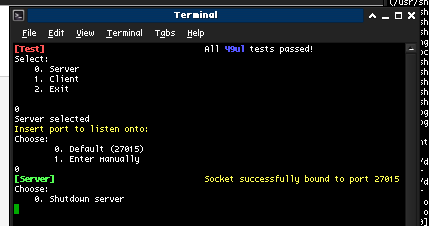
\includegraphics[width=0.5\textwidth]{screen1}
                \end{figure}

                When the application is running in server mode, the only possible user command is the shutdown of the application itself.
                Everything else is handled automatically.

                Information is displayed on sent/received data and client connections/disconnections.


            \subsection{Client role}
        
                \begin{figure}[h]
                \caption{Example of the chat application being ran in client mode.}
                \centering
                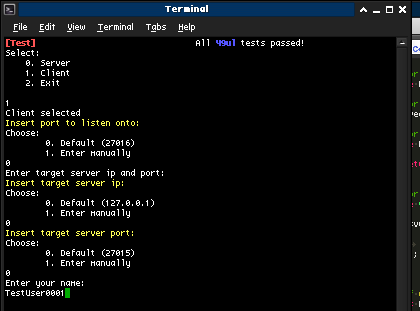
\includegraphics[width=0.5\textwidth]{screen2}
                \end{figure}

                When the application is running in client mode, after successfully connecting to the server, the user can interact in several ways.

                \begin{itemize}
                  \item Messages can be created and sent to the server.
                  \item A request to edit an existing message on the server can be sent.
                  \item The current local state of the client can be displayed.
                \end{itemize}

                

    \newpage

    HOW TO GET, COSE, GITHUB, WEBSITE, DEPENDENCIES

\end{document}
